%!TEX root=../main.tex
\section{Programming and Computation Model}
\label{sec:programming-model}
We introduce \SystemName{}, which realizes above design principles via following programming and computation model. 




\begin{figure}[t]
\centering
% \scriptsize
\begin{lstlisting}[
    caption={The declarative programming model of \SystemName{}.
    },
    label={list:api-example-1}
]
import rollart.distributed as rdist
from rdist.worker import AcrtorTrainCls, ActorGenCls, RewardCls
from rdist import ResourceManager as RM

# 1. Single Controller Example
class MyActorTrain(ActorTrainCls):
    @rdist.register(mode="execute_all")
    def compute_gradients(self, input_tensor):
        ...

# 2. Define actor_gen on heterogeneous GPUs
# 2.1 heterogeneous GPU allocation. 
gen_rm=RM( {"H800": list(range(0, 8))},  
           {"H20", list(range(8, 32))})
# 2.2 hardware affinity mapping
class HeteroActorGen(ActorGenCls):
    @rdist.hw_mapping(
    hw_affinity={"FrozenLake": "H800","default": "H20"}
    )
    def generate(self, input_ids:List[int], 
                tag_name:str="default"):
        return self.model.process(prompt)

# 3. Define a serverless reward computation func
class ServerlessRewardWorker(RewardCls):
    @rdist.register_serverless(
        attribute='reward_proxy',
        serverless_url='fc://xxx.xxx')
    def compute_rewards(self, traj: list):
        prompt = f"Evaluate the trajectory:{traj}"
        return ray.get(self.reward_proxy(prompt))

    
\end{lstlisting}
% \vspace{-15pt}
\end{figure}




\subsection{Declarative Programming Model}
In the runtime, a worker is the minimum unit to own resources. \autoref{list:api-example-1} shows the programming model defined at the worker function level, giving the runtime fine-grained visibility into resource usage. The details are as follows.



\noindent\textbf{Single Controller.} This programming model is widely adopted in industrial RL frameworks~\cite{verl,slime_github} as it streamlines the construction of agentic RL pipelines. \SystemName{} adopts this model and realizes it via the \texttt{register} decorator. When the execution mode is set to \texttt{execute\_all} (Lines~7-8 in \autoref{list:api-example-1}), the runtime broadcasts inputs to all trainer workers and invokes \texttt{compute\_gradients} on each worker. \SystemName{} manages distributed computation and communication across workers, while users implement the computation logic inside each execution function and compose the agentic training pipeline by invoking execution functions of different types of workers. 



\noindent\textbf{Hardware-Affinity Mapping (Principle 1).} \SystemName{} supports provisioning heterogeneous resource groups through a dictionary-based resource specification (Lines~13–14). The detailed illustration of the resource manager can be found in \S\ref{sec:architecture}. We use the \texttt{generate} function in the \texttt{HeteroActorGen} class (Lines~16-22) to illustrate how to declare fine-grained, affinity-aware hardware mappings for a worker method via the \texttt{hw\_mapping} decorator (Lines~17–19). Specifically, LLM generation workloads tagged as \texttt{FrozenLake} are routed with high priority to compute-optimized GPUs, while other workloads are routed with high priority to bandwidth-optimized GPUs. The \texttt{tag\_name} argument (Line~21) serves as a dynamic routing hint, allowing each LLM generation request to be automatically dispatched to workers bound to the appropriate hardware. This routing mechanism ensures that each trajectory generation executes with effective resource affinity.

\noindent\textbf{Serverless Registration (Principle 3).} \SystemName{} exposes \texttt{register\_serverless} (Lines~26-28) to declare the statefulness of an execution method. This decorator allows the runtime to invoke \texttt{compute\_rewards} (Line~29) as a pure function on a serverless worker pool via the specified \texttt{serverless\_url}. The serverless platform automatically manages resource provisioning, scaling, and request routing to achieve high resource efficiency.


% The new code listing
\begin{figure}[t]
\centering
\begin{lstlisting}[
    caption={The simplfied implementation and of \texttt{Cluster} and its running example in \SystemName{}.},
    label={list:api-example-cluster}
]
class Cluster: 
    def __init__(self, res_manager, worker_cls): 
        self._create_worker(worker_cls, res_manager)
        self._bind_worker_method()
    
    def execute_all(self, method_name, *args, **kwargs):
        result = []
        for worker in self.workers: 
            rcall = getattr(worker, method_name)
            result.append(rcall(*args, **kwargs))
        return ray.get(result)

    def hw_mapping(self, hw_affinity, tag_name, *args):
        hw_type = hw_affinity.get(tag_name)
        new_workers = []
        for worker in self.workers:
            if worker.resource_type == hw_type: 
                new_workers.append(worker)
        # route requests to new_workers next

    def register_serverless(self, attr, url, *args): 
        # define a call_fc to call serverless url
        for worker in self.workers: 
            setattr(worker, attr, call_fc)
        # perform execute_all logic next
\end{lstlisting}
\end{figure}



\subsection{Key Abstraction: \texttt{Cluster}}
\label{sec:cluster}
The above programming model simplifies the development of agentic RL training.
We next discuss how it is implemented via our \texttt{Cluster} abstraction (in \autoref{list:api-example-cluster}). Specifically, this abstraction is implemented to serve as a controller, managing the execution of distributed workers across RL stages. 


\PHM{Distributed Workers.}
The \texttt{Worker} serves as the fundamental execution unit in \SystemName{}. 
As a base class, it can be specialized into various computational units for different roles (e.g., training, generation) required across the stages.
The \texttt{Cluster} instantiates a set of workers according to the specified \texttt{worker\_cls}, and uses the resource manager to allocate resources to each worker and label their resource types for hardware affinity mapping (Line 3 in \autoref{list:api-example-cluster}). The resource manager owns and manages a collection of resources. 

\PHM{Invocation Proxy.} The \texttt{\_bind\_worker\_method} function binds each method of the specified \texttt{worker\_cls} to the \texttt{Cluster} instance, allowing the \texttt{Cluster} to act as a proxy for the corresponding collection of workers (Line~4). For example, if \texttt{worker\_cls} defines a method \texttt{compute\_gradients}, users can directly invoke \texttt{Cluster.compute\_gradients}.

We now describe the computation model underlying our programming model. First, to realize the single controller mechanism, when users invoke a method annotated with the \texttt{register} decorator, \SystemName{} enters the \texttt{execute\_all} method, which calls the target method on all workers and aggregates their results (Liness~6-11). Second, for methods annotated with \texttt{hw\_mapping}, \SystemName{} inspects the \texttt{tag\_name} argument, filters for workers bound to the preferred resource type, and executes the method on those selected workers (Lines 13–19). Third, for methods annotated with \texttt{register\_serverless}, the reward proxy (\texttt{attr}) is replaced with the registered serverless url, so reward computation is performed by a serverless function (Lines 21–25). We discuss prefill–decoding disaggregation and asynchronous cross-cluster weight update next. 



\noindent\textit{\underline{Prefill–Decoding Disaggregation.}} Many systems~\cite{distserve, patel2023splitwise} disaggregate prefill and decoding across heterogeneous GPUs. During rollout, the \texttt{Cluster} allows distributed workers to leverage these engines to realize such disaggregation. However, real deployments currently require manual configuration of prefill and decoding instances, which easily leads to load imbalance. We hence leave it as future work. 

% Automating this within \SystemName{} is left to future work.


% \textcolor{cyan}{ Tianyuan:
\noindent\textit{\underline{Asynchronous Cross-Cluster Weight Update.}} Hardware-affinity-driven disaggregation requires cross-cluster communication between the rollout (e.g., H20) and training (e.g., H800) clusters, which may be physically separated and connected only via low-bandwidth Ethernet links. This slow interconnect can become a bottleneck for weight update in frameworks designed for a single, uniform high-bandwidth network~\cite{verl}. \SystemName{} addresses this by implementing an asynchronous weight update engine using Mooncake~\cite{qin2024mooncake}. In our design, training workers (on the H800 cluster) asynchronously publish weights to the Mooncake store without waiting for the concurrent rollout stage to finish, while inference workers (on the H20 cluster) can fetch them on-demand. Then, we follow the existing approach~\cite{verl} to perform model update within clusters. By effectively hiding cross-cluster communication overhead behind ongoing trajectories, the asynchronous cross-cluster weight update can reduce the end-to-end training overhead. 

\begin{figure}
    \centering
    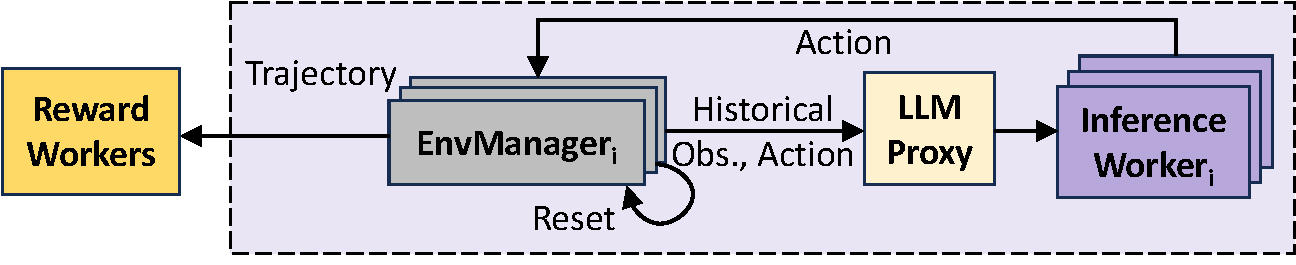
\includegraphics[width=\linewidth]{figs/overview/traj-level-rollout.pdf}
    \vspace{-10pt}
    \caption{Trajectory-Level Rollout Overview.}
    \label{fig:traj_rollout}
\end{figure}

\subsection{Asynchronous Workflows}
\label{subsec:async-workflow}
We describe the asynchronous workflows in \SystemName{} that realize fine-grained asynchrony (\textbf{Principle 2}). Within rollout, LLM generation is overlapped with environment execution. Across stages, rollout is overlapped with reward and training.

\PHM{\texttt{LLMProxy}: Trajectory-Level LLM Generation.} \texttt{LLMProxy} is a gateway that decouples LLM serving clients from the underlying serving instances. It intelligently orchestrates requests across a fleet of internal LLM inference workers. Each worker is built around a command-driven event loop that manages an inference engine (e.g., vLLM~\cite{vllm}, SGLang~\cite{sglang}).

This loop runs continuously in a non-blocking fashion with two components:  
(1) \textit{Step-wise command processing.} The loop continuously polls for commands dispatched from \texttt{LLMProxy}, \texttt{ADD} to enqueue new requests and \texttt{ABORT} to cancel existing ones. When no commands are pending, it advances the inference engine by executing a single decode or prefill step for a batch of requests, keeping GPU utilization high. This design ensures that adding or aborting an ongoing trajectory does not stall the entire LLM generation process.  (2) \textit{Post-processing.} When the LLM engine finishes a request after a certain prefill/decoding step, the loop immediately invokes a pre-registered callback. This callback post-processes the output and returns the result to the original client (e.g., an \texttt{EnvManager}). This allows each trajectory to perform environment interaction as soon as its LLM generation completes, without waiting for stragglers. Together, both functions enable trajectory-level LLM generation. 




\PHM{\texttt{EnvManager}: Trajectory-level Environment Interaction.} Each \texttt{EnvManager} is a lightweight controller that manages the lifecycle of a single environment to collect trajectories, as shown in \autoref{fig:traj_rollout}. It begins with environment initialization via \texttt{reset}, after which it enters an independent event loop that orchestrates the interaction between an environment instance and the shared \texttt{LLMProxy}. During this loop, the \texttt{EnvManager} maintains a list of (observation, action) pairs to construct a trajectory. Specifically, it feeds \texttt{LLMProxy} with the historical (observation, action) sequence as input to obtain the next action, applies this action to the environment via \texttt{step}, and records the resulting observation. % This loop repeats until a termination criterion is met. 

In practice, \SystemName{} launches multiple \texttt{EnvManager} instances simultaneously, and each \texttt{EnvManager} yields a single trajectory rather than batch-executing environment interactions (as shown in \autoref{fig:sub-batched_env_interaction}). As a result, long-tail environment workers do not delay the execution of other workers. Combined with trajectory-level LLM generation, \SystemName{} can overlap LLM generation with environment interaction in a fine-grained manner. Furthermore, upon completing a trajectory, the \texttt{EnvManager} immediately invokes a reward computation function via a serverless API as a non-blocking task, allowing reward computation to overlap with ongoing rollouts. Overall, this trajectory-level rollout management enables a high degree of parallelism to maximize throughput. 


\begin{figure}
    \centering
    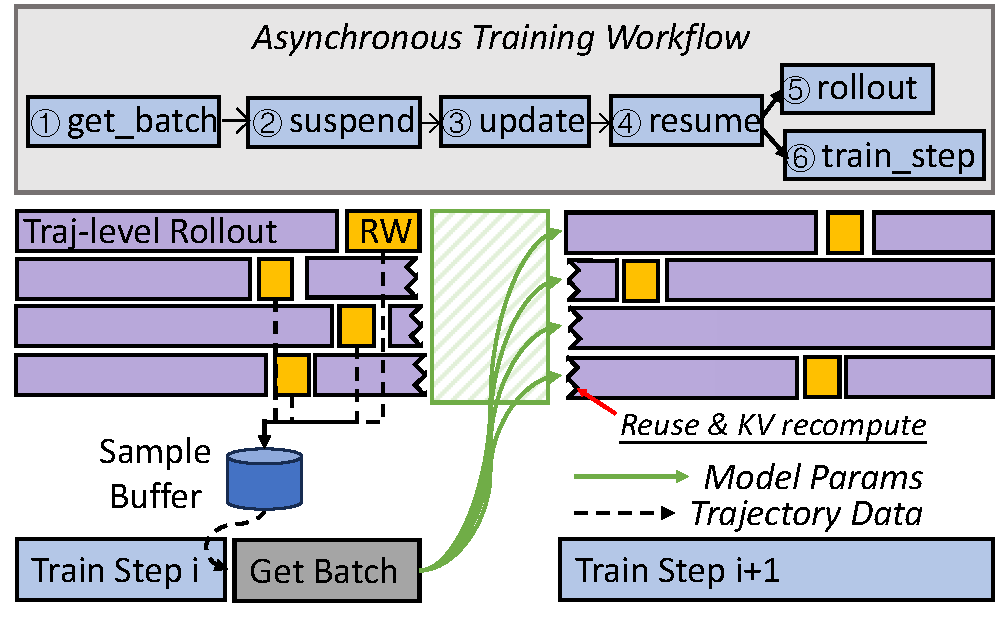
\includegraphics[width=0.9\linewidth]{figs/overview/rollout_scheduler_osdi_resume.pdf}
    % \vspace{-10pt}
    \caption{Asynchronous Training Workflow.}
    \label{fig:rollout_scheduler}
\end{figure}

\noindent\textit{\underline{Optimization: Redundant Env Rollouts.}}  
The trajectory-level design of \texttt{LLMProxy} and \texttt{EnvManager} enables an optimization we term \textit{redundant environment rollouts}. This technique allows users to launch more environments than strictly required to interact with the agent LLM. Once the target number of trajectories has been collected, any ongoing rollouts can be terminated and even aborted. Because rollouts are managed at the trajectory level, slow environments do not block or delay faster ones. This effectively mitigates fail-slow and fail-stop environments. 
Our empirical analysis in \S\ref{subsec:eval-async} reveals that this technique improves rollout efficiency.
Furthermore, large-scale deployments in \S\ref{sec:large-scale-analysis} benefit from this by avoiding the impact of environment failures.


\PHM{Asynchronous Training Workflow.}
\autoref{fig:rollout_scheduler} shows how \SystemName{} orchestrates the asynchronous training workflow. In the rollout stage, multiple \texttt{EnvManager}s act independently, continuously 
% interacting with \texttt{LLMProxy} to generate 
generating trajectories and enqueue them into the \texttt{SampleBuffer}. LLM inference and training workers run on separate GPUs, enabling disaggregated training.

The training workflow periodically runs a weight synchronization protocol. It first invokes a blocking \texttt{get\_batch} call to retrieve a batch of trajectories from the \texttt{SampleBuffer}. It then issues a \texttt{suspend} command to halt trajectory collection, performs a \texttt{model\_update} by fetching the latest LLM and broadcasting its weights to all inference workers.
This process is accelerated by the non-blocking, cross-cluster communication optimization detailed in \S\ref{sec:cluster}.
Subsequently, it issues a \texttt{resume} command to continue the trajectory-level rollout with the updated model.
\emph{Unfinished trajectories from the previous iteration are also reused in the current one, through 
KV cache recomputation}. Last, it executes \texttt{train\_step} on the retrieved data. In asynchronous training mode, the training stage overlaps with the rollout stage, and \SystemName{} controls the staleness of a trajectory with asynchronous bound.


\PHM{Asynchronous Bound.}
In asynchronous training, trajectory generation can be interrupted and later resumed under a newer agent LLM. Thus, a single batch of trajectories may be generated by multiple versions of LLM. The staleness introduces high variance and compromise training stability. AReaL~\cite{areal} addresses this by constraining the average sample freshness within each batch to preserve model quality. Differently, \SystemName{} introduces an \textbf{asynchronous bound} $\alpha$ to regulate freshness at the per-trajectory level and to actively manage the asynchronous workflow. It is defined per trajectory as the maximum allowable gap in version numbers between the current agent LLM and the version that initiated generation of that trajectory. If the agent LLM has advanced to version $n$, then any trajectory in \texttt{SampleBuffer} must have been initiated by a version no older than $(n - \alpha)$. Trajectories that violate this constraint are aborted. Our empirical study (\S\ref{ssec:e2e-performance}) suggests that setting the asynchronous bound to one yields a balance between training speed and stability.

